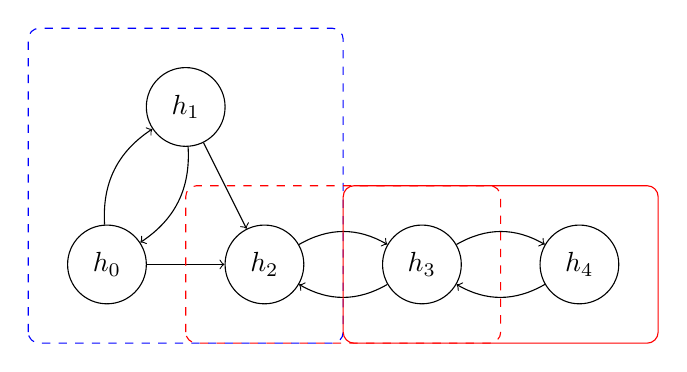
\begin{tikzpicture}[neuron/.style={circle, minimum size=1cm, draw=black!100}]
    \draw[rounded corners, blue, dashed] (0, 0) rectangle (4, 4);
    
    \node[neuron] (h-1) at (2, 3) {$h_1$};
    \node[neuron] (h-0) at (1, 1) {$h_0$};
    \node[neuron] (h-2) at (3, 1) {$h_2$};
    
    \draw[->] (h-0) edge [bend left] (h-1);
    \draw[->] (h-1) edge [bend left] (h-0);
    \draw[->] (h-1) -- (h-2);
    \draw[->] (h-0) -- (h-2);
    
    \draw[rounded corners, red, dashed] (2, 0) rectangle (6, 2);
    
    \node[neuron] (h-3) at (5, 1) {$h_3$};
    
    \draw[->] (h-2) edge [bend left] (h-3);
    \draw[->] (h-3) edge [bend left] (h-2);

    \draw[rounded corners, red] (4, 0) rectangle (8, 2);

    \node[neuron] (h-4) at (7, 1) {$h_4$};
    
    \draw[->] (h-3) edge [bend left] (h-4);
    \draw[->] (h-4) edge [bend left] (h-3);
\end{tikzpicture}
